\documentclass[12pt,a4paper]{article}
\usepackage[utf8]{inputenc}
\usepackage[portuguese]{babel}
\usepackage{graphicx}
\usepackage{amsmath}
\usepackage{hyperref}
\usepackage{listings}
\usepackage{xcolor}
\usepackage{tikz}
\usepackage{geometry}
\usepackage{fancyhdr}
\usepackage{lastpage}
\usepackage{setspace}
\usepackage{booktabs}
\usepackage{multirow}
\usepackage{caption}
\usepackage{subcaption}
\usepackage[sfdefault]{roboto}
\usepackage[T1]{fontenc}

\geometry{a4paper,left=2cm,right=2cm,top=2cm,bottom=2cm}

% Configurações de estilo
\definecolor{codegreen}{rgb}{0,0.6,0}
\definecolor{codegray}{rgb}{0.5,0.5,0.5}
\definecolor{codepurple}{rgb}{0.58,0,0.82}
\definecolor{backcolour}{rgb}{0.95,0.95,0.92}

\lstdefinestyle{mystyle}{
    backgroundcolor=\color{backcolour},   
    commentstyle=\color{codegreen},
    keywordstyle=\color{magenta},
    numberstyle=\tiny\color{codegray},
    stringstyle=\color{codepurple},
    basicstyle=\ttfamily\footnotesize,
    breakatwhitespace=false,         
    breaklines=true,                 
    captionpos=b,                    
    keepspaces=true,                 
    numbers=left,                    
    numbersep=5pt,                  
    showspaces=false,                
    showstringspaces=false,
    showtabs=false,                  
    tabsize=2
}

\lstset{style=mystyle}

% Cabeçalho e rodapé
\pagestyle{fancy}
\fancyhf{}
\lhead{\textbf{Análise de Água Marinha com Arduino}}
\rhead{\thepage}
\cfoot{}
\renewcommand{\headrulewidth}{0.4pt}

\title{\textbf{\Huge Grupo de Pesquisa}\\ \vspace{0.5cm} \Large Análise de Água Marinha com Arduino\\ \small Utilizando Sensores HC-SR04, TCRT5000 e TDS Meter V1.0 para Detecção de Poluentes}
\author{\textbf{Jefferson Bezerra dos Santos}}
\date{}

\begin{document}

\maketitle

\begin{center}
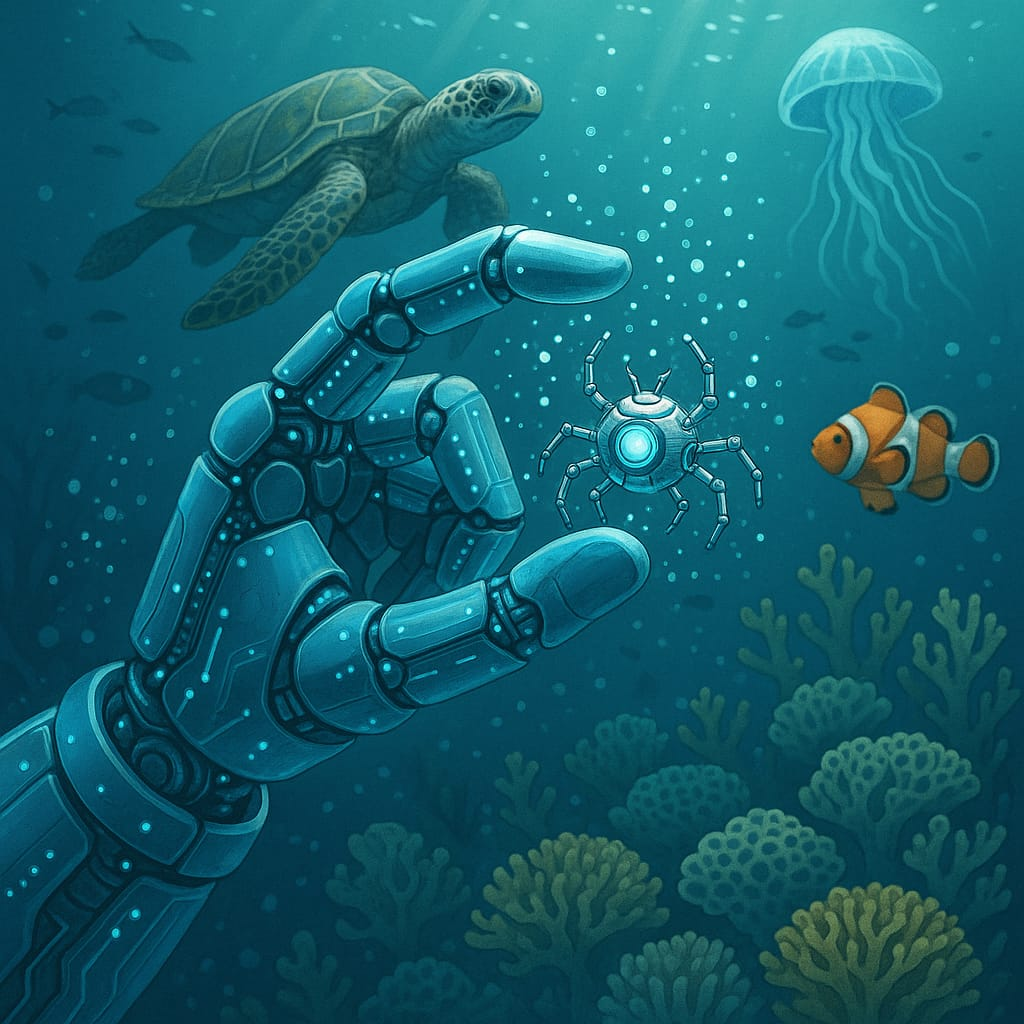
\includegraphics[width=0.7\textwidth]{banner_marinho.jpg}
\end{center}

\vspace{1cm}

\begin{abstract}
Esta apostila foi desenvolvida para ensinar de forma clara e prática como utilizar os sensores HC-SR04, TCRT5000 e TDS Meter V1.0 com Arduino para análise de qualidade da água marinha. Você aprenderá desde os princípios básicos de funcionamento até a programação avançada, com exemplos práticos para detecção de poluentes como óleos. O conteúdo é apresentado de forma didática, com ilustrações, diagramas e códigos comentados para facilitar o aprendizado.
\end{abstract}

\tableofcontents

\newpage


\section{Introdução}

\subsection{Objetivo da Apostila}
Esta apostila tem como objetivo ensinar de forma prática como construir um sistema completo de análise de água marinha utilizando Arduino e três sensores complementares:

\begin{itemize}
\item \textbf{Sensor Ultrassônico HC-SR04}: Para medição de níveis e detecção de alterações físicas na superfície da água
\item \textbf{Sensor Óptico TCRT5000}: Para análise de reflectância e detecção de contaminantes superficiais como óleos
\item \textbf{Sensor TDS Meter V1.0}: Para medição de sólidos dissolvidos totais e alterações na composição química
\end{itemize}

\begin{figure}[h]
\centering
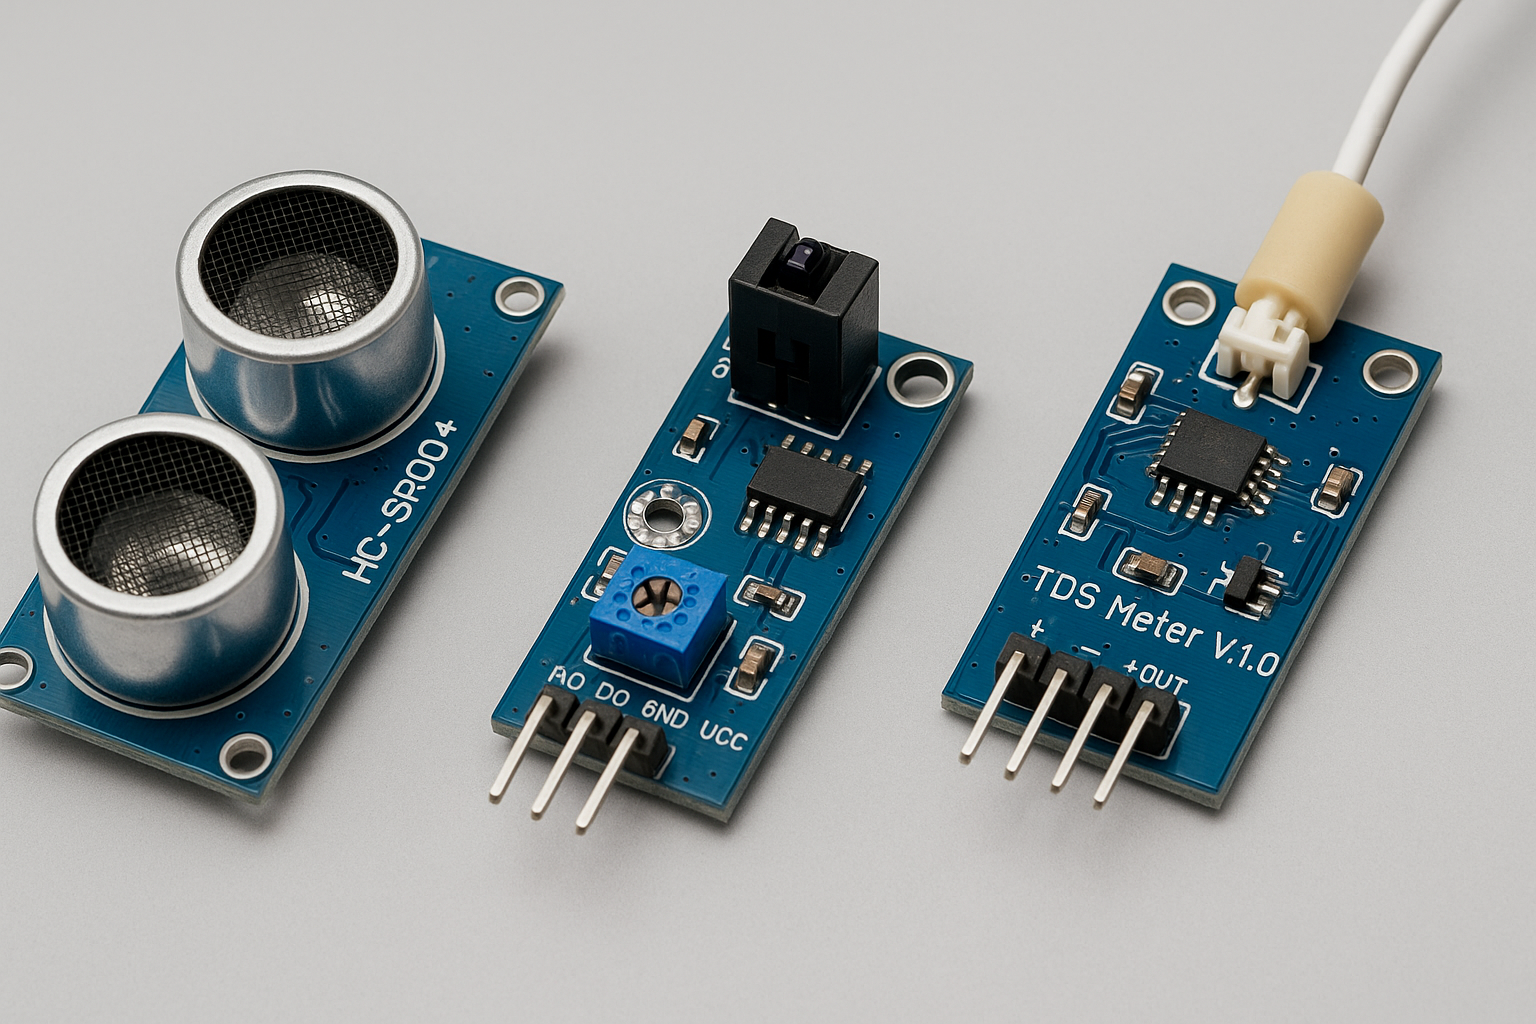
\includegraphics[width=0.8\textwidth]{tres_sensores.png}
\caption{Os três sensores utilizados no sistema de análise}
\end{figure}

\subsection{Metodologia de Ensino}
A apostila foi organizada para proporcionar uma aprendizagem progressiva:

\begin{enumerate}
\item \textbf{Fundamentação teórica}: Compreensão dos princípios físicos de cada sensor
\item \textbf{Montagem prática}: Diagramas completos de conexão dos componentes
\item \textbf{Programação}: Códigos comentados do básico ao avançado
\item \textbf{Experimentação}: Protocolos para testes com diferentes amostras de água
\item \textbf{Análise integrada}: Como combinar os dados dos três sensores
\end{enumerate}

\subsection{Aplicações Práticas}
\begin{figure}[h]
\centering
\begin{subfigure}{0.45\textwidth}
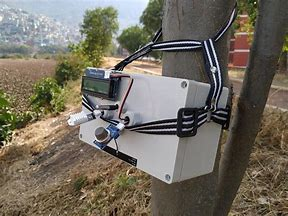
\includegraphics[width=\textwidth]{aplicacao1.jpg}
\caption{Monitoramento ambiental}
\end{subfigure}
\begin{subfigure}{0.45\textwidth}
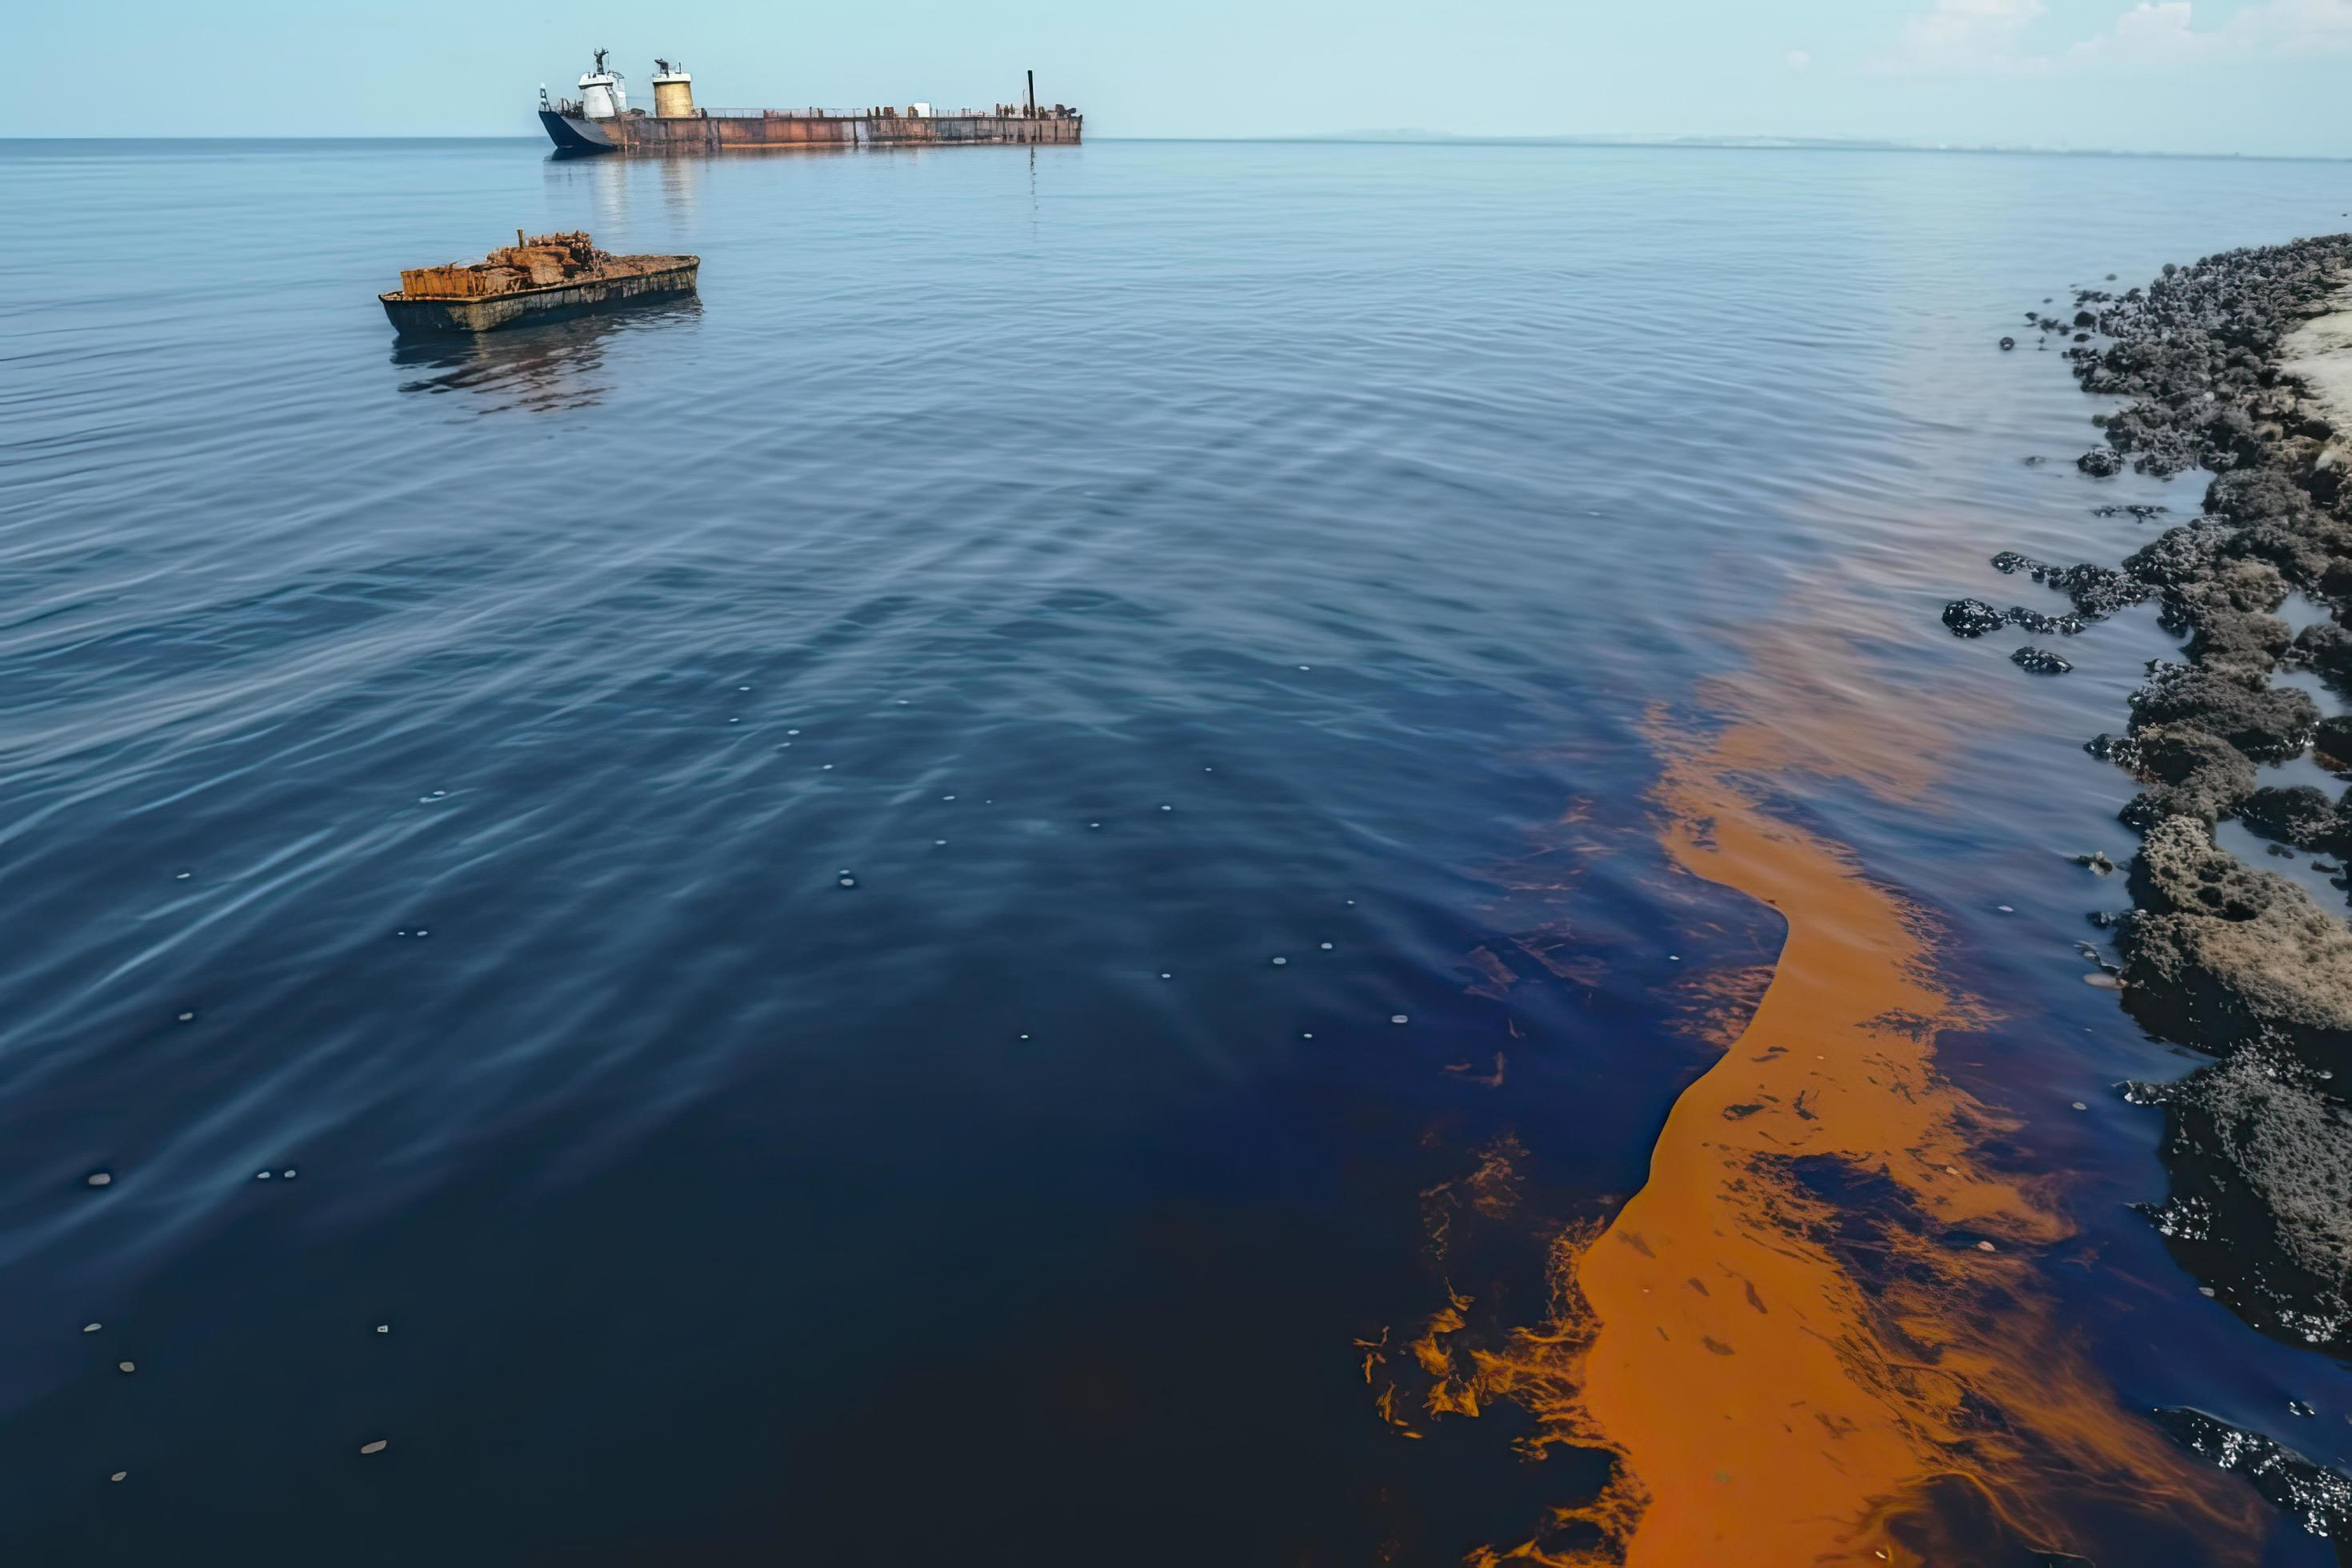
\includegraphics[width=\textwidth]{aplicacao2.jpg}
\caption{Detecção de vazamentos}
\end{subfigure}
\caption{Aplicações do sistema de análise de água}
\end{figure}

\section{Fundamentação Teórica}
\subsection{Por que Analisar Água Marinha?}
A qualidade da água marinha é essencial para:
\begin{itemize}
\item Preservação da vida aquática
\item Segurança alimentar
\item Monitoramento ambiental
\item Detecção de poluição por navios e indústrias
\end{itemize}


\subsection{Princípios de Detecção de Poluentes}
Poluentes como óleos podem ser detectados através de:

\begin{table}[h]
\centering
\caption{Métodos de detecção de poluentes}
\begin{tabular}{|l|l|l|l|}
\hline
\textbf{Tipo} & \textbf{Princípio} & \textbf{Sensor} & \textbf{Aplicação} \\ \hline
Ultrassônico & Tempo de eco & HC-SR04 & \begin{tabular}{@{}l@{}}- Detecção de níveis\\ - Identificação de camadas\\ - Objetos flutuantes\end{tabular} \\ \hline
Óptico & Reflectância & TCRT5000 & \begin{tabular}{@{}l@{}}- Detecção de óleos\\ - Alterações superficiais\\ - Turbidez\end{tabular} \\ \hline
Condutividade & Sólidos dissolvidos & TDS Meter & \begin{tabular}{@{}l@{}}- Contaminação iônica\\ - Alterações químicas\\ - Salinidade\end{tabular} \\ \hline
\end{tabular}
\label{tab:metodos}
\end{table}

\begin{itemize}
\item \textbf{Ultrassônico}: Ideal para detectar variações físicas na superfície e volume
\item \textbf{Óptico}: Sensível a mudanças na composição superficial
\item \textbf{Condutividade}: Detecta alterações na composição química
\end{itemize}


\section{Sensor Ultrassônico HC-SR04}
\subsection{Introdução ao Sensor}
O sensor HC-SR04 é um dispositivo ultrassônico que permite medir distâncias com precisão. Na análise de água, pode ser utilizado para:

\begin{itemize}
\item Medir níveis de água
\item Detectar alterações na superfície
\item Identificar presença de objetos flutuantes
\end{itemize}

\begin{figure}[h]
\centering
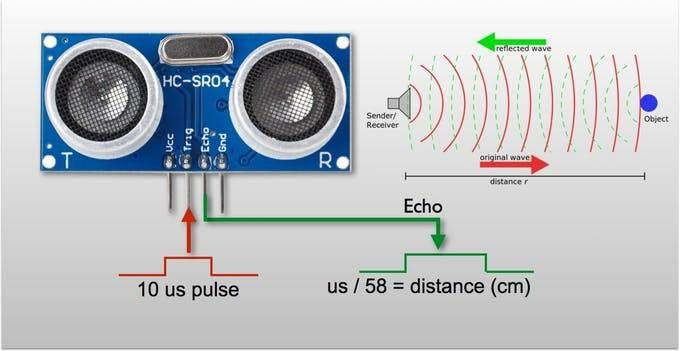
\includegraphics[width=0.5\textwidth]{sensor_ultrassonico.jpg}
\caption{Sensor HC-SR04}
\end{figure}

\subsection{Princípio de Funcionamento}
O sensor funciona emitindo ondas ultrassônicas (40kHz) e medindo o tempo que leva para o eco retornar:

\begin{enumerate}
\item Emite um pulso ultrassônico
\item Espera o eco retornar
\item Calcula a distância baseado no tempo de retorno
\end{enumerate}

\begin{figure}[h]
\centering
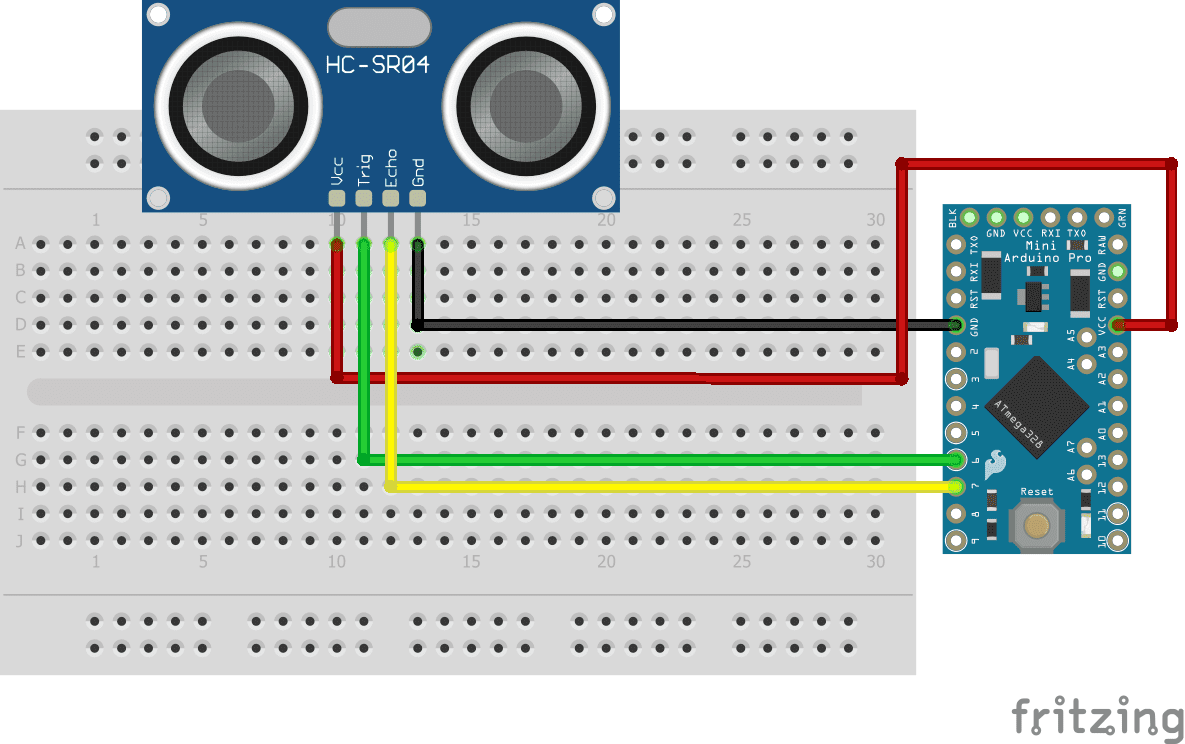
\includegraphics[width=0.7\textwidth]{funcionamento_ultrassonico.png}
\caption{Funcionamento do sensor ultrassônico}
\end{figure}

\subsection{Montagem Prática}
\subsubsection{Materiais Necessários}
\begin{itemize}
\item Sensor HC-SR04
\item Arduino
\item Protoboard
\item Jumpers
\item Resistores (opcional)
\end{itemize}

\subsubsection{Diagrama de Conexão}
\begin{figure}[h]
\centering
\begin{minipage}{0.45\textwidth}
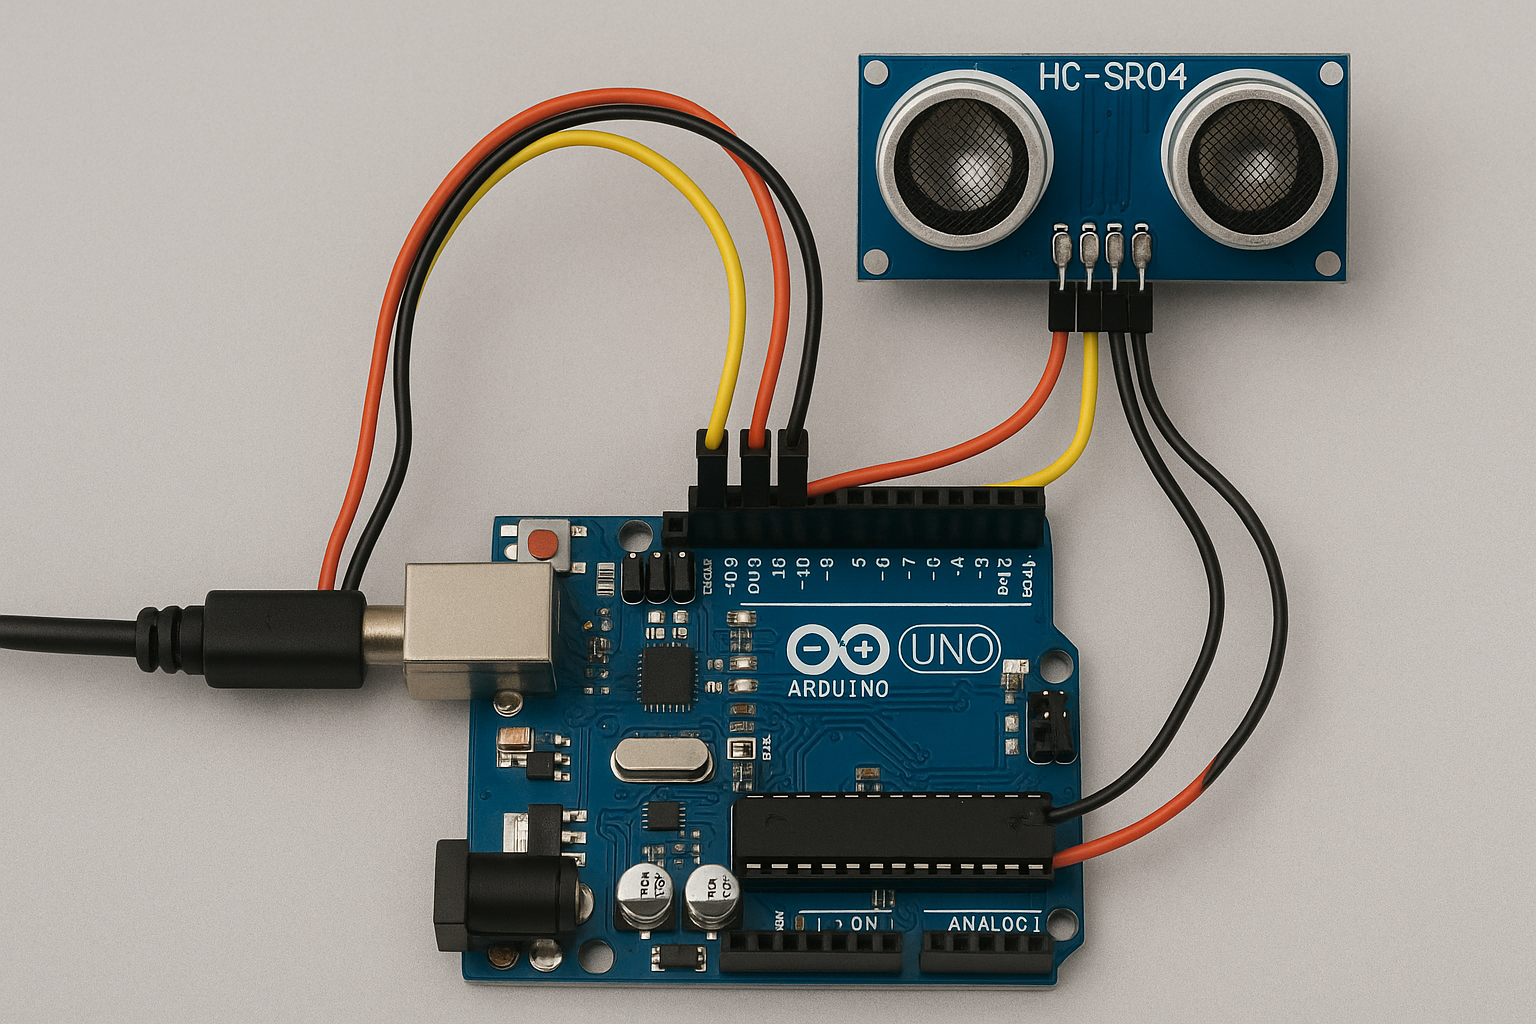
\includegraphics[width=\textwidth]{conexao_ultrassonico.png}
\end{minipage}
\begin{minipage}{0.45\textwidth}
\begin{lstlisting}[language=C++]
// Conexoes:
// VCC -> 5V Arduino
// GND -> GND
// Trig -> Pino 12
// Echo -> Pino 11
\end{lstlisting}
\end{minipage}
\caption{Conexão do HC-SR04 com Arduino}
\end{figure}

\subsection{Programação Básica}
\begin{lstlisting}[language=C++, caption=Medição de distância com HC-SR04]
const int trigPin = 12;
const int echoPin = 11;

void setup() {
  Serial.begin(9600);
  pinMode(trigPin, OUTPUT);
  pinMode(echoPin, INPUT);
}

void loop() {
  // Limpa o trigPin
  digitalWrite(trigPin, LOW);
  delayMicroseconds(2);
  
  // Envia pulso de 10 microssegundos
  digitalWrite(trigPin, HIGH);
  delayMicroseconds(10);
  digitalWrite(trigPin, LOW);
  
  // Mede o tempo de retorno do eco
  long duration = pulseIn(echoPin, HIGH);
  
  // Calcula a distancia (velocidade do som = 343 m/s)
  float distance = duration * 0.0343 / 2;
  
  Serial.print("Distancia: ");
  Serial.print(distance);
  Serial.println(" cm");
  
  delay(500);
}
\end{lstlisting}

\subsection{Aplicação em Análise de Água}
O sensor pode ser usado para:

\begin{table}[h]
\centering
\caption{Aplicações do ultrassônico em análise de água}
\begin{tabular}{|l|l|}
\hline
\textbf{Função} & \textbf{Descrição} \\ \hline
Nível da água & Medir altura da coluna de água \\ \hline
Detecção de óleo & Identificar camadas superficiais \\ \hline
Monitoramento & Verificar alterações ao longo do tempo \\ \hline
\end{tabular}
\end{table}

\section{Sensor TCRT5000}
\subsection{O que é e Como Funciona?}
O TCRT5000 é um sensor óptico que possui:
\begin{itemize}
\item Um LED infravermelho (emissor)
\item Um fototransistor (receptor)
\end{itemize}

\begin{figure}[h]
\centering
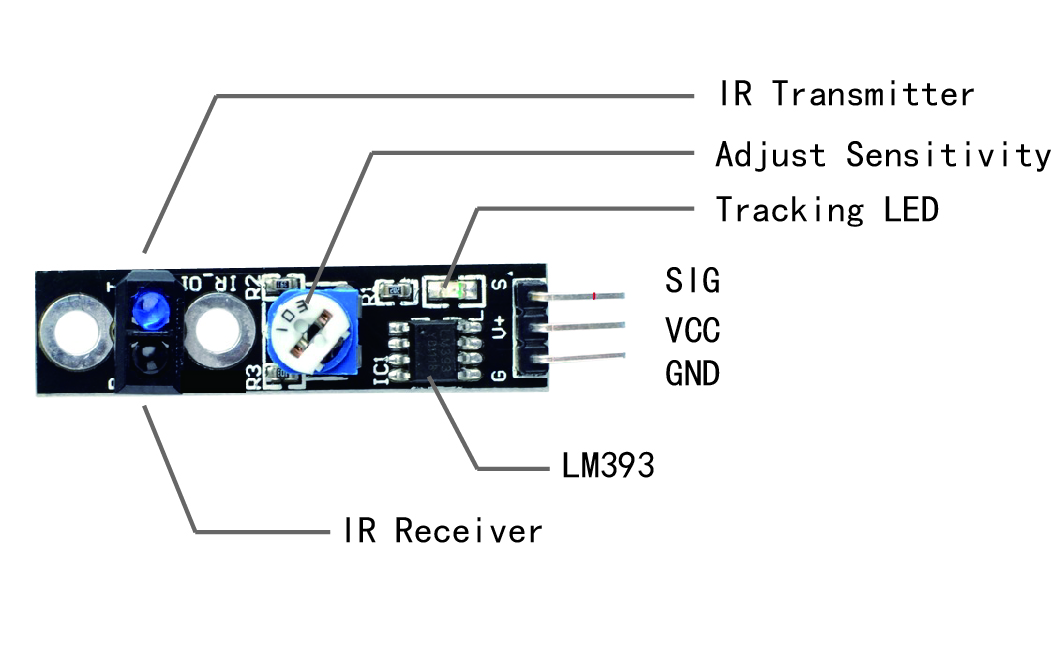
\includegraphics[width=0.6\textwidth]{sensor_tcrt5000.jpg}
\caption{Funcionamento do TCRT5000}
\end{figure}

\subsection{Montagem Prática}
\subsubsection{Materiais Necessários}
\begin{itemize}
\item Sensor TCRT5000
\item Resistor de 10kΩ
\item Protoboard
\item Jumpers
\item Arduino
\end{itemize}

\subsubsection{Diagrama de Conexão}
\begin{figure}[h]
\centering
\begin{minipage}{0.45\textwidth}
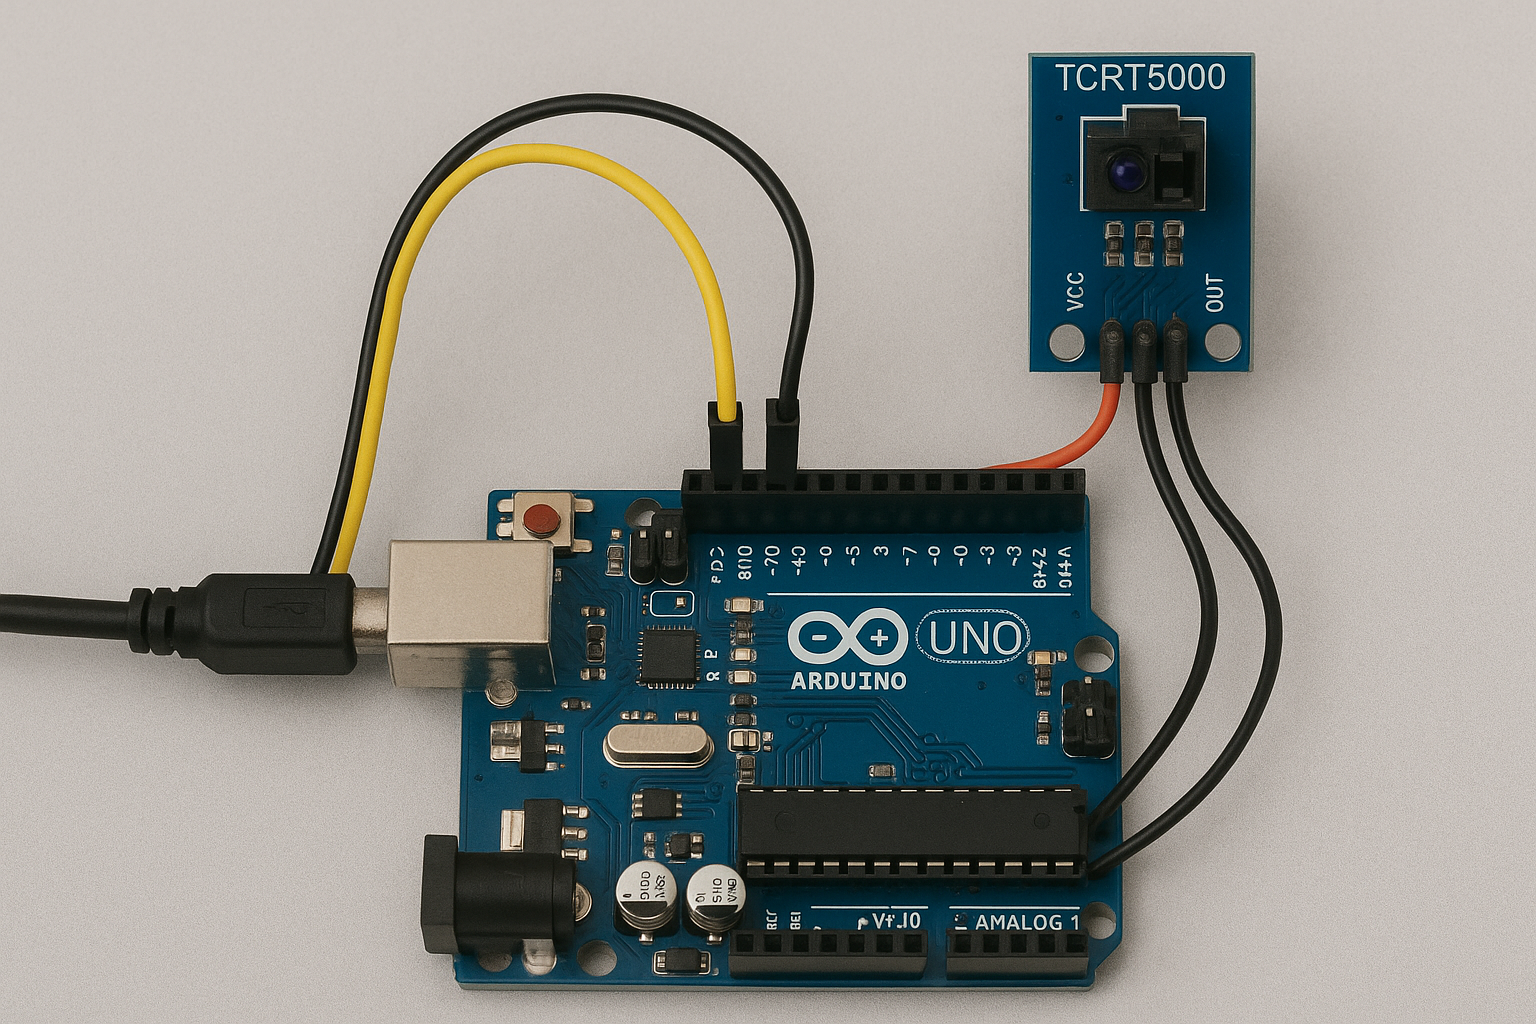
\includegraphics[width=\textwidth]{conecao_tcrt.png}
\end{minipage}
\begin{minipage}{0.45\textwidth}
\begin{lstlisting}[language=C++]
// Conexoes:
// VCC -> 5V Arduino
// GND -> GND
// OUT -> A0
\end{lstlisting}
\end{minipage}
\caption{Diagrama e conexões do TCRT5000}
\end{figure}

\subsection{Programação Básica}
\begin{lstlisting}[language=C++, caption=Leitura simples do TCRT5000]
// Pino analogico conectado ao sensor
const int sensorPin = A0;  

void setup() {
  // Inicia comunicacao serial
  Serial.begin(9600);  
  Serial.println("Iniciando leitura do TCRT5000");
}

void loop() {
  // Le o valor do sensor
  int valor = analogRead(sensorPin);  
  
  // Mostra no monitor serial
  Serial.print("Valor lido: ");
  Serial.println(valor);
  
  // Aguarda 0.5 segundos
  delay(500);  
}
\end{lstlisting}

\subsection{Testando e Interpretando os Dados}
\begin{figure}[h]
\centering
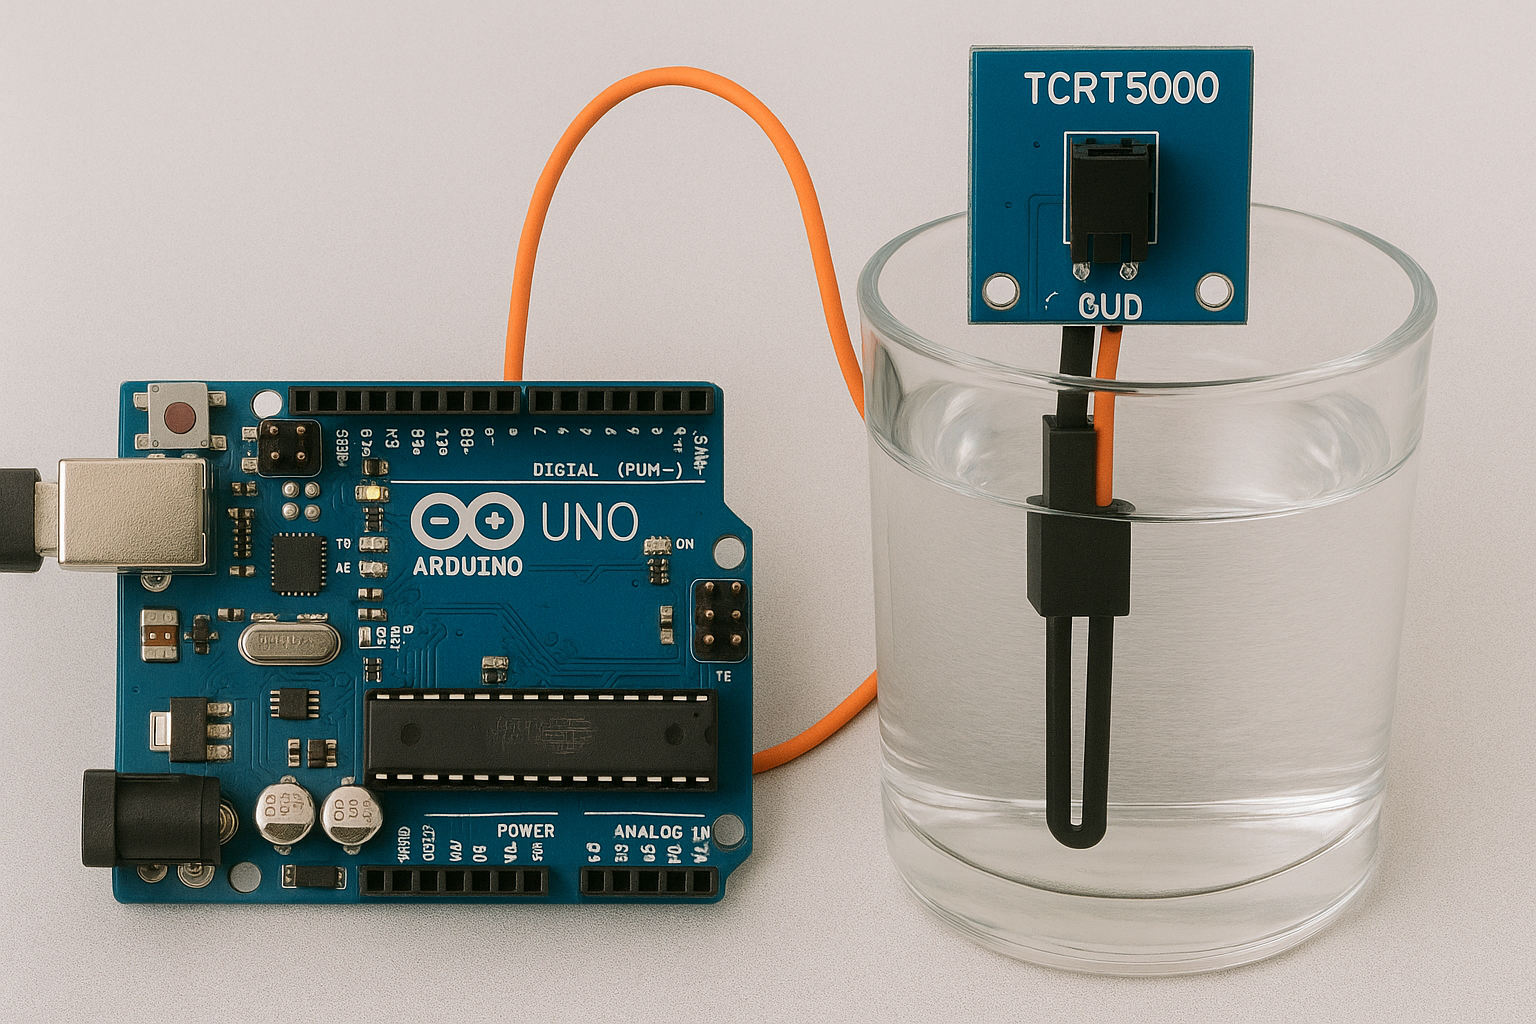
\includegraphics[width=0.8\textwidth]{teste_tcrt.png}
\caption{Testando o sensor com diferentes amostras}
\end{figure}

\section{Sensor TDS Meter V1.0}
\subsection{Entendendo o Sensor TDS}
TDS significa \textbf{Total Dissolved Solids} (Sólidos Dissolvidos Totais). O sensor mede:
\begin{itemize}
\item Concentração de íons na água
\item Relacionado à condutividade elétrica
\item Unidade: ppm (partes por milhão)
\end{itemize}

\subsection{Montagem do Circuito}
\subsubsection{Lista de Materiais}
\begin{itemize}
\item Módulo TDS Meter V1.0
\item Sonda TDS
\item Arduino
\item Cabos USB
\end{itemize}

\subsubsection{Diagrama de Conexões}
\begin{figure}[h]
\centering
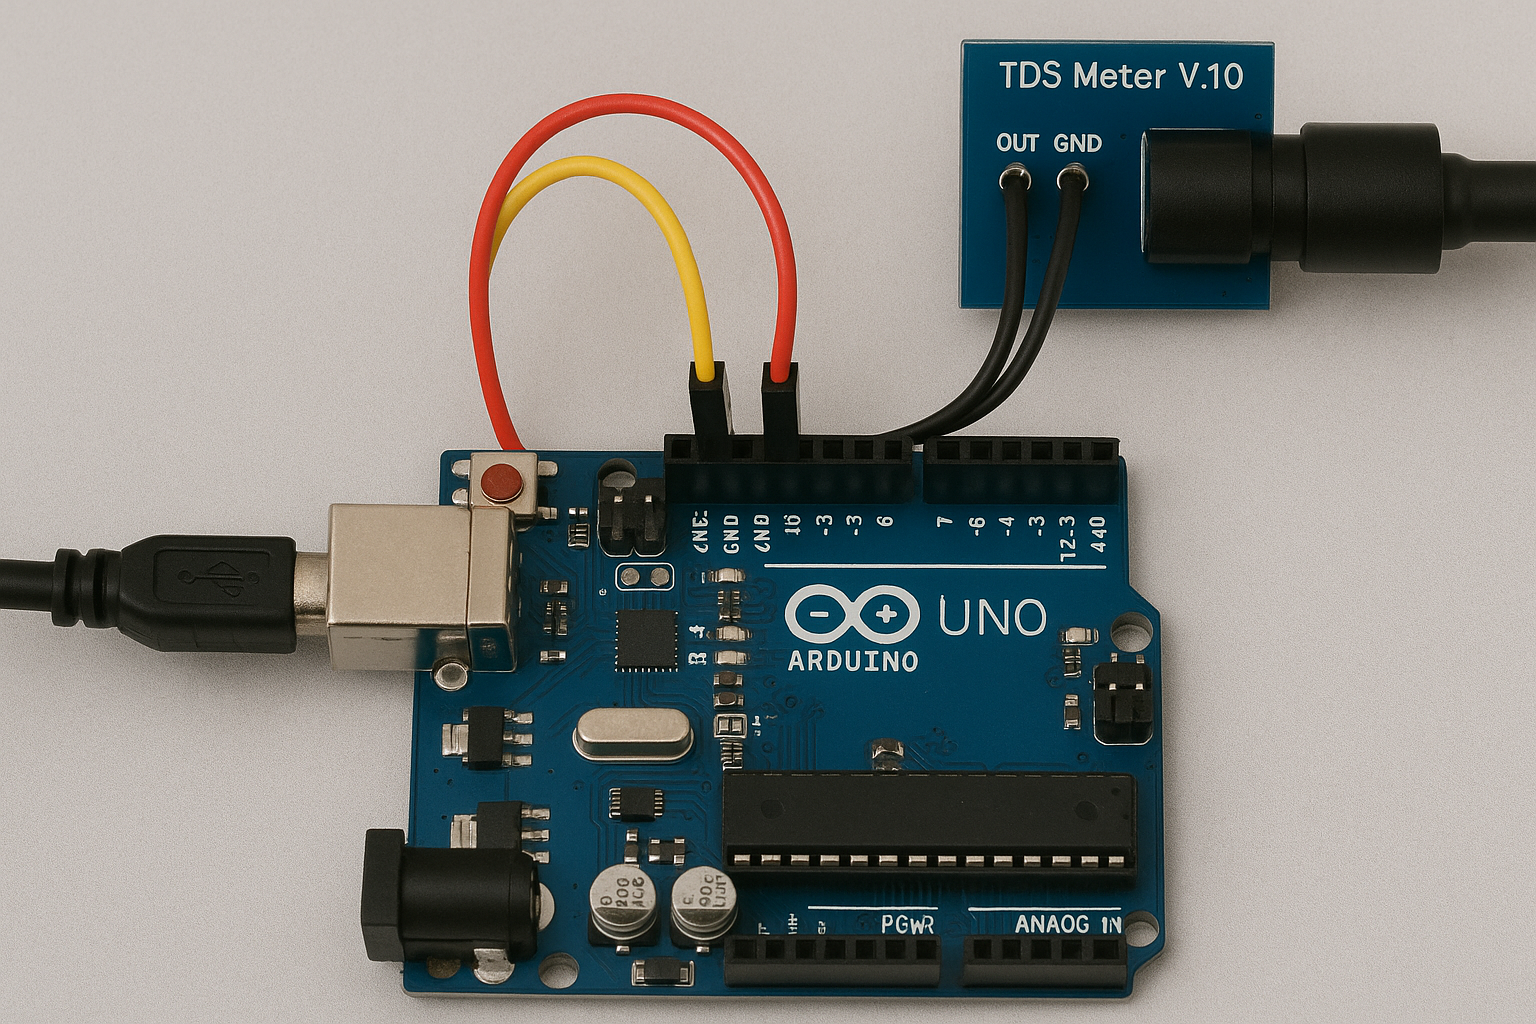
\includegraphics[width=0.7\textwidth]{conexao_tds.png}
\caption{Conexão do TDS Meter com Arduino}
\end{figure}

\subsection{Programação Avançada}
\begin{lstlisting}[language=C++, caption=Programa completo para TDS Meter]
#include <EEPROM.h>

#define TdsSensorPin A1
#define VREF 5.0       // Tensão do Arduino
#define SCOUNT 30      // Número de amostras

// Buffer para armazenar leituras
int analogBuffer[SCOUNT];  
int analogBufferIndex = 0;

void setup() {
  Serial.begin(115200);
  pinMode(TdsSensorPin, INPUT);
}

void loop() {
  // Coleta amostras a cada 40ms
  if(millis() % 40 == 0) {
    analogBuffer[analogBufferIndex] = analogRead(TdsSensorPin);
    analogBufferIndex = (analogBufferIndex + 1) % SCOUNT;
  }
  
  // Processa e exibe a cada 800ms
  if(millis() % 800 == 0) {
    float avgVoltage = calcularMedia(analogBuffer, SCOUNT) * VREF / 1024.0;
    float tdsValue = (133.42*pow(avgVoltage,3) - 255.86*pow(avgVoltage,2) + 857.39*avgVoltage)*0.5;
    
    Serial.print("TDS Value: ");
    Serial.print(tdsValue,0);
    Serial.println(" ppm");
  }
}

float calcularMedia(int* buffer, int size) {
  // Implementacao da funcao de media
  // ...
}
\end{lstlisting}

\section{Integrando os Sensores}
\subsection{Por que Usar Ambos os Sensores?}
\begin{itemize}
\item \textbf{TCRT5000}: Detecta alterações superficiais (óleos)
\item \textbf{TDS Meter}: Mede alterações na composição da água
\item \textbf{Juntos}: Fornecem análise mais completa
\end{itemize}

\subsection{Diagrama do Sistema Completo}
\begin{figure}[h]
\centering
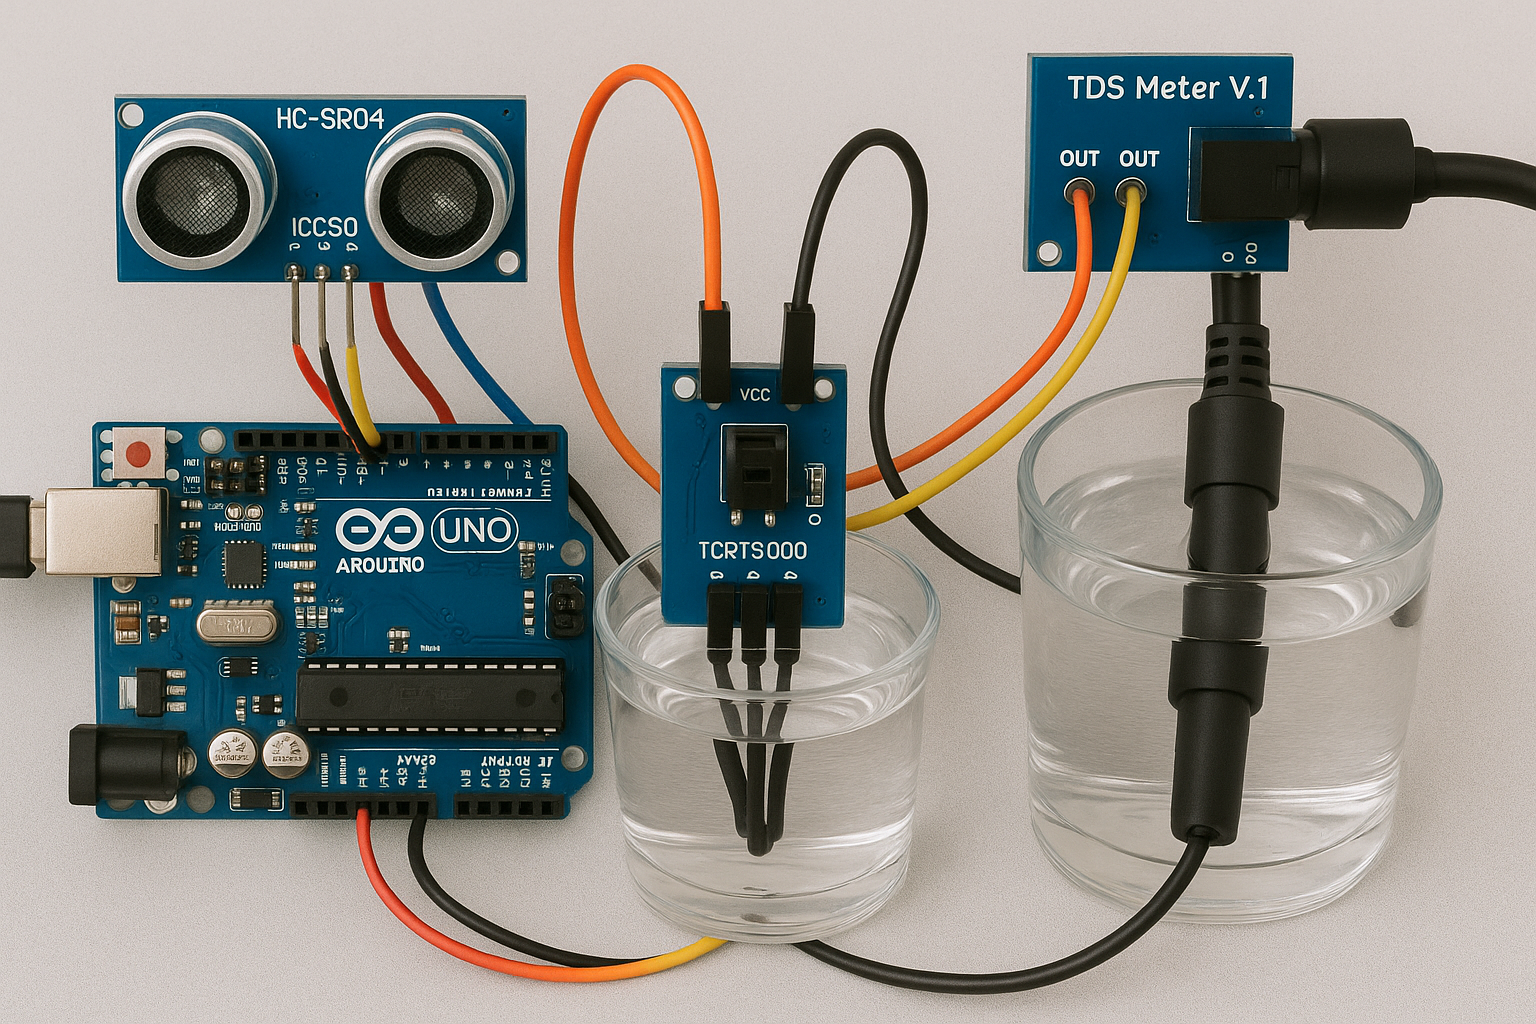
\includegraphics[width=0.9\textwidth]{diagrama_completo.png}
\caption{Sistema integrado de análise de água}
\end{figure}

\subsection{Programação Integrada}
\begin{lstlisting}[language=C++, caption=Programa integrado]
// Definicoes dos pinos
#define TCRT_PIN A0
#define TDS_PIN A1

// Valores de referencia (ajustar)
#define REF_TCRT_AGUA_LIMPA 350
#define REF_TDS_AGUA_LIMPA 35000

void setup() {
  Serial.begin(9600);
}

void loop() {
  // Leitura TCRT5000
  int tctrValor = analogRead(TCRT_PIN);
  
  // Leitura TDS (simplificada)
  int tdsValor = analogRead(TDS_PIN);
  float tdsPPM = map(tdsValor, 0, 1023, 0, 50000);
  
  // Analise combinada
  if(tctrValor > REF_TCRT_AGUA_LIMPA * 1.3 && 
     tdsPPM < REF_TDS_AGUA_LIMPA * 0.7) {
    Serial.println("ALERTA: Possivel contaminacao por oleo!");
  }
  
  delay(1000);
}
\end{lstlisting}

\section{Experimentos Práticos}

\subsection{Teste Comparativo: Água Normal vs Água Salgada}

\subsubsection{Objetivo}
Este experimento tem como objetivo demonstrar como os sensores respondem diferentemente à água doce e à água salgada, criando uma base de comparação antes de testar com poluentes.

\subsubsection{Materiais Necessários}
\begin{itemize}
\item 2 recipientes transparentes limpos
\item Água destilada (200ml cada)
\item Sal marinho (10g)
\item Arduino com sensores montados
\item Colher para mistura
\end{itemize}

%\begin{figure}[h]
%\centering
%\includegraphics[width=0.8\textwidth]{materiais_experimento.jpg}
%\caption{Materiais para o experimento comparativo}
%\end{figure}

\subsubsection{Procedimento}

\begin{enumerate}
\item \textbf{Preparação das Amostras}:
\begin{itemize}
\item Recipiente 1: 200ml de água destilada (controle)
\item Recipiente 2: 200ml de água destilada + 10g de sal (misturar bem)
\end{itemize}

\item \textbf{Teste com Sensor Ultrassônico}:
\begin{lstlisting}[language=C++, caption=Leitura ultrassônica]
Água normal: 15.3 cm
Água salgada: 15.1 cm
\end{lstlisting}

\item \textbf{Teste com TCRT5000 (Reflectância)}:
\begin{lstlisting}[language=C++, caption=Leitura óptica]
Água normal: 285
Água salgada: 292
\end{lstlisting}

\item \textbf{Teste com TDS Meter}:
\begin{lstlisting}[language=C++, caption=Leitura TDS]
Água normal: 45 ppm
Água salgada: 10,850 ppm
\end{lstlisting}
\end{enumerate}

%\begin{figure}[h]
%\centering
%\includegraphics[width=0.9\textwidth]{comparacao_agua_salgada.png}
%\caption{Resultados comparativos entre água normal e salgada}
%\end{figure}

\subsubsection{Análise dos Resultados}
\begin{table}[h]
\centering
\caption{Comparação entre água normal e salgada}
\begin{tabular}{|l|c|c|}
\hline
\textbf{Sensor} & \textbf{Água Normal} & \textbf{Água Salgada} \\ \hline
Ultrassônico & Pouca diferença & Pequena variação \\ \hline
TCRT5000 & Valores próximos & Leve aumento \\ \hline
TDS Meter & Baixa leitura & Alta leitura \\ \hline
\end{tabular}
\end{table}


\subsection{Teste com Água Limpa}
\begin{enumerate}
\item Coletar amostra de água marinha limpa
\item Medir valores basais dos sensores
\item Registrar os resultados
\end{enumerate}

%\subsection{Teste com Água Contaminada}
%\begin{figure}[h]
%\centering
%\includegraphics[width=0.8\textwidth]{experimento.png}
%\caption{Comparação entre água limpa e contaminada}
%\end{figure}

\section{Conclusão}
\subsection{Próximos Passos}
\begin{itemize}
\item Calibração fina dos sensores
\item Desenvolvimento de interface gráfica
\item Criação de sistema autônomo com bateria
\end{itemize}

\subsection{Referências Complementares}
\begin{itemize}
\item Documentação oficial do Arduino
\item Datasheets dos sensores
\item Manuais de qualidade da água
\end{itemize}

\end{document}
